\section{Identification des demandes des parties}
\subsection{Objectif de la tâche}
\begin{frame}[c]{\mysubsectiontitle}
Extraction de données sur les demandes des parties
\begin{itemize} \scriptsize 
	\item Exemple : demande de dommage-intérêts pour procédure abusive
	%danais/CASAI1401082.xml
	\begin{itemize} \scriptsize 
		\item Extrait de décision relatif à la demande: 
\fbox{\parbox{0.8\textwidth}{\tiny
	Jennifer M. et Catherine M. ... demandent à la Cour de :
	
	- \textcolor{red}{infirmer le dit jugement} en \textcolor{blue}{toutes ses dispositions} ; 
	...
	
	Statuant à nouveau ...
	
	- les condamner au paiement d'une somme de  \textbf{3 000,00 \euro{} pour procédure abusive} et
	aux entiers dépens ; ...
	
	La cour ... CONFIRME \textcolor{red}{le jugement entrepris} en \textcolor{blue}{toutes ses dispositions}.}}
	\textit{\tiny Légende : référence au jugement antérieur en \textcolor{red}{rouge}, énoncés fusionnés en \textcolor{blue}{bleue}}
    \item Données à extraire       
	\end{itemize}
\end{itemize}
 \centering{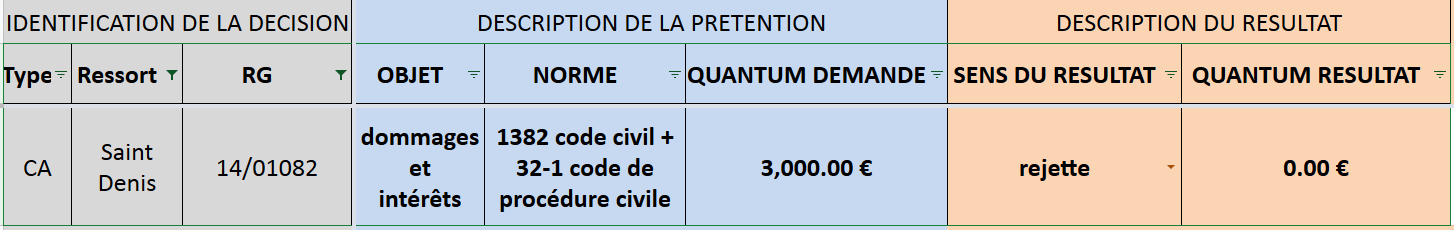
\includegraphics[width=\textwidth]{tab-danais.png}}
 
 \vspace{-0.2cm}
 \begin{itemize} \scriptsize 
\item Difficultés
	\begin{itemize}\scriptsize 
		\item Présence de plusieurs demandes de catégories similaires et/ou différentes dans une même décision
		\item Toutes les catégories ne sont pas connues d'avance (+500 catégories)
		\item Difficile d'annoter une base d'évaluation pour toutes les couvrir
		%\item Énonces non structurés, avec des références, et des agrégations
	\end{itemize}
\end{itemize}
\end{frame}

\subsection{Méthode proposée : approche par catégorie de demandes}

\begin{frame}[t]{\mysubsectiontitle}
	Extraction d'une seule catégorie ($c$) à l'aide de sa terminologie
	
	\begin{itemize} \scriptsize	
		\item Détection de la présence de la catégorie par classification de la décision ($c$ vs. $\overline{c}$)
		%\item Identification des passages de demandes (section Litige) et résultats (section Dispositif)
		\item Identification des quantas : montants à proximité des termes-clés de $c$ dans les énoncés explicites de demandes et résultats		

		\fbox{\parbox{0.8\textwidth}{\scriptsize
				Jennifer M. et Catherine M. ... demandent à la Cour de :
				
				- infirmer le dit jugement en toutes ses dispositions ; 
				...
				
				Statuant à nouveau ...
				
				- \textbf{[} les condamner au paiement d' une somme de  \fbox{\parbox{0.13\textwidth}{\textit{\fontfamily{qcs}\selectfont{3 000,00 \euro}}}}  \textbf{pour procédure abusive} et
				aux entiers dépens ; \textbf{]}$_\text{demande\_danais}$ ...
			
			La cour ... CONFIRME le jugement entrepris en toutes ses dispositions.}}
		
	    \item Identification du sens du résultat 
	    \begin{itemize} \scriptsize
	    	\item soit en fonction du verbe introductif de l'énoncé du résultat	 
	    	\begin{tabular}{|p{0.34\textwidth}|p{0.22\textwidth}|p{0.22\textwidth}|}
	    		\hline
 \multicolumn{3}{|c|}{\textbf{Résultat} (par polarité)} \\ \hline
	    		\textbf{accepte}  &\textbf{sursis à statuer} & \textbf{rejette}  \\ \hline
 \textit{accorde, admet, condamne, ...} & \textit{réserve, surseoit, ...} & \textit{déboute, rejette, ...} \\ \hline
	    	\end{tabular}   	
	    	\item soit \textit{"rejette"} si pas d'énoncé explicite du résultat
	    \end{itemize}
		\item Mise en correspondance des informations relatives à la même demande
		\begin{itemize} \scriptsize
			\item énoncé demande et énoncé résultat similaires
			\item quantum demandé et quantum accordé apparaissant dans le même ordre
		\end{itemize}
	\end{itemize}
\end{frame}

\begin{frame}[t]{\mysubsectiontitle}
	Apprentissage de la catégorie à extraire
	\begin{itemize} \scriptsize
		\item Entraînement d'un algorithme de classification pour détecter sa présence 
		\item Détermination automatique de sa terminologie à l'aide d'une méthode de pondération de termes : 
		\begin{itemize} \scriptsize
			\item $idf(t) = \log_2\left(\frac{N}{N_t}\right)$ \cite{sparck1972idf}
			\item $\Delta_{DF}(t,c) = DF_{t \vert c} - DF_{t \vert \overline{c}}$
			\item $\chi^2(t,c) = \frac{N ((N_{t,c} N_{\overline{t},\overline{c}}) - (N_{t,\overline{c}} N_{\overline{t},c}))^2}{N_t N_{\overline{t}} \vert D_c \vert \vert D_{\overline{c}} \vert }$ \cite{schutze1995chi2}
			\item $ngl(t,c) = \frac{\sqrt{N} (N_{t,c} N_{\overline{t},\overline{c}}) - (N_{t,\overline{c}} N_{\overline{t},c})}{\sqrt{N_t N_{\overline{t}} \vert D_c \vert \vert D_{\overline{c}} \vert }}$ \cite{ng1997ngl}
			\item etc.
		\end{itemize}
	\end{itemize}
\end{frame}
\subsection{Résultats expérimentaux}
\begin{frame}[t]{\mysubsectiontitle}
	Catégories sur lesquelles la méthode a été expérimentée
	
	\scriptsize
		\begin{tabular}{|c|p{0.35\textwidth}|p{0.15\textwidth}|p{0.3\textwidth}|}
			\hline
			\textbf{Label} & \textbf{Nom} & \textbf{Objet} & \textbf{Fondement} \\ \hline
			\textit{acpa} & amende civile pour abus de procédure & amende civile & Articles 32-1 code de procédure civile + 559 code de procédure civile \\ \hline
			\textit{concdel} & dommages-intérêts pour concurrence déloyale & dommages-intérêts & Article 1382 du code civil \\ \hline
			\textit{danais} & dommages-intérêts pour abus de procédure & dommages-intérêts & Articles 32-1 code de procédure civile + 1382 code de procédure civile \\ \hline
			\textit{dcppc} & déclaration de créance au passif de la procédure collective & déclaration de créance & L622-24 code de commerce \\ \hline
			\textit{doris} & dommages-intérêts pour trouble de voisinage & dommages-intérêts & principe de responsabilité pour trouble anormal de voisinage \\ \hline
			\textit{styx} & frais irrépétibles & dommages-intérêts & Article 700 du code de procédure civile \\ \hline
		\end{tabular}
\end{frame}
\begin{frame}[t]{\mysubsectiontitle}
	Quantité de décisions annotées manuellement par l'expert
	
	\centering	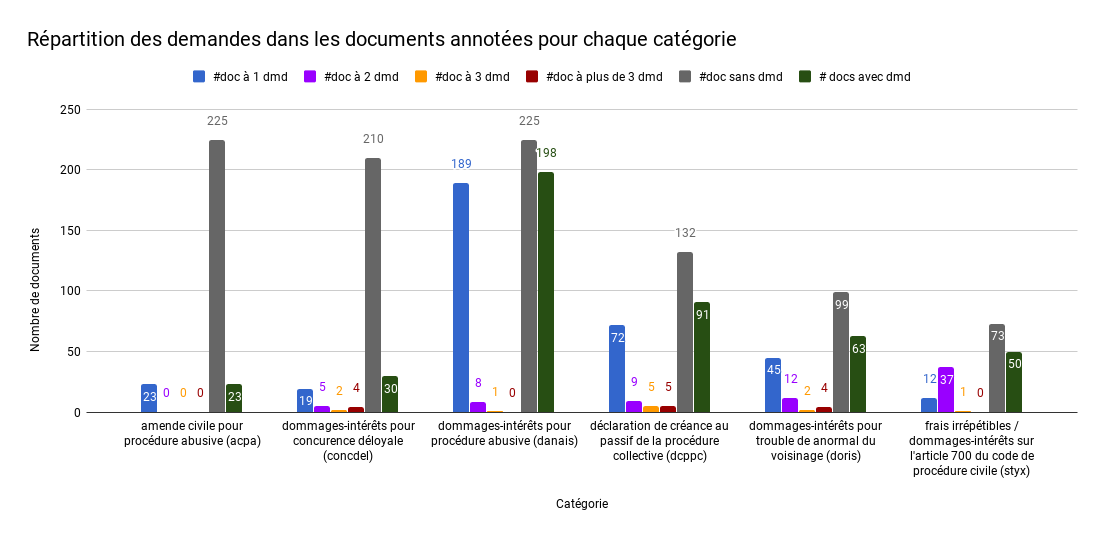
\includegraphics[width=0.8\textwidth]{chartDataset.png}
\end{frame}


\begin{frame}[t]{\mysubsectiontitle}
	Efficacité de la méthode
	\begin{itemize} \scriptsize
		\item Les algorithmes traditionnels (KNN, SVM, naïf bayésien, arbre) donnent de bons résultats pour la détection de la catégorie : $98.8\% \leq F_1 \leq 100\%$
		\item Extraction :
		{\centering{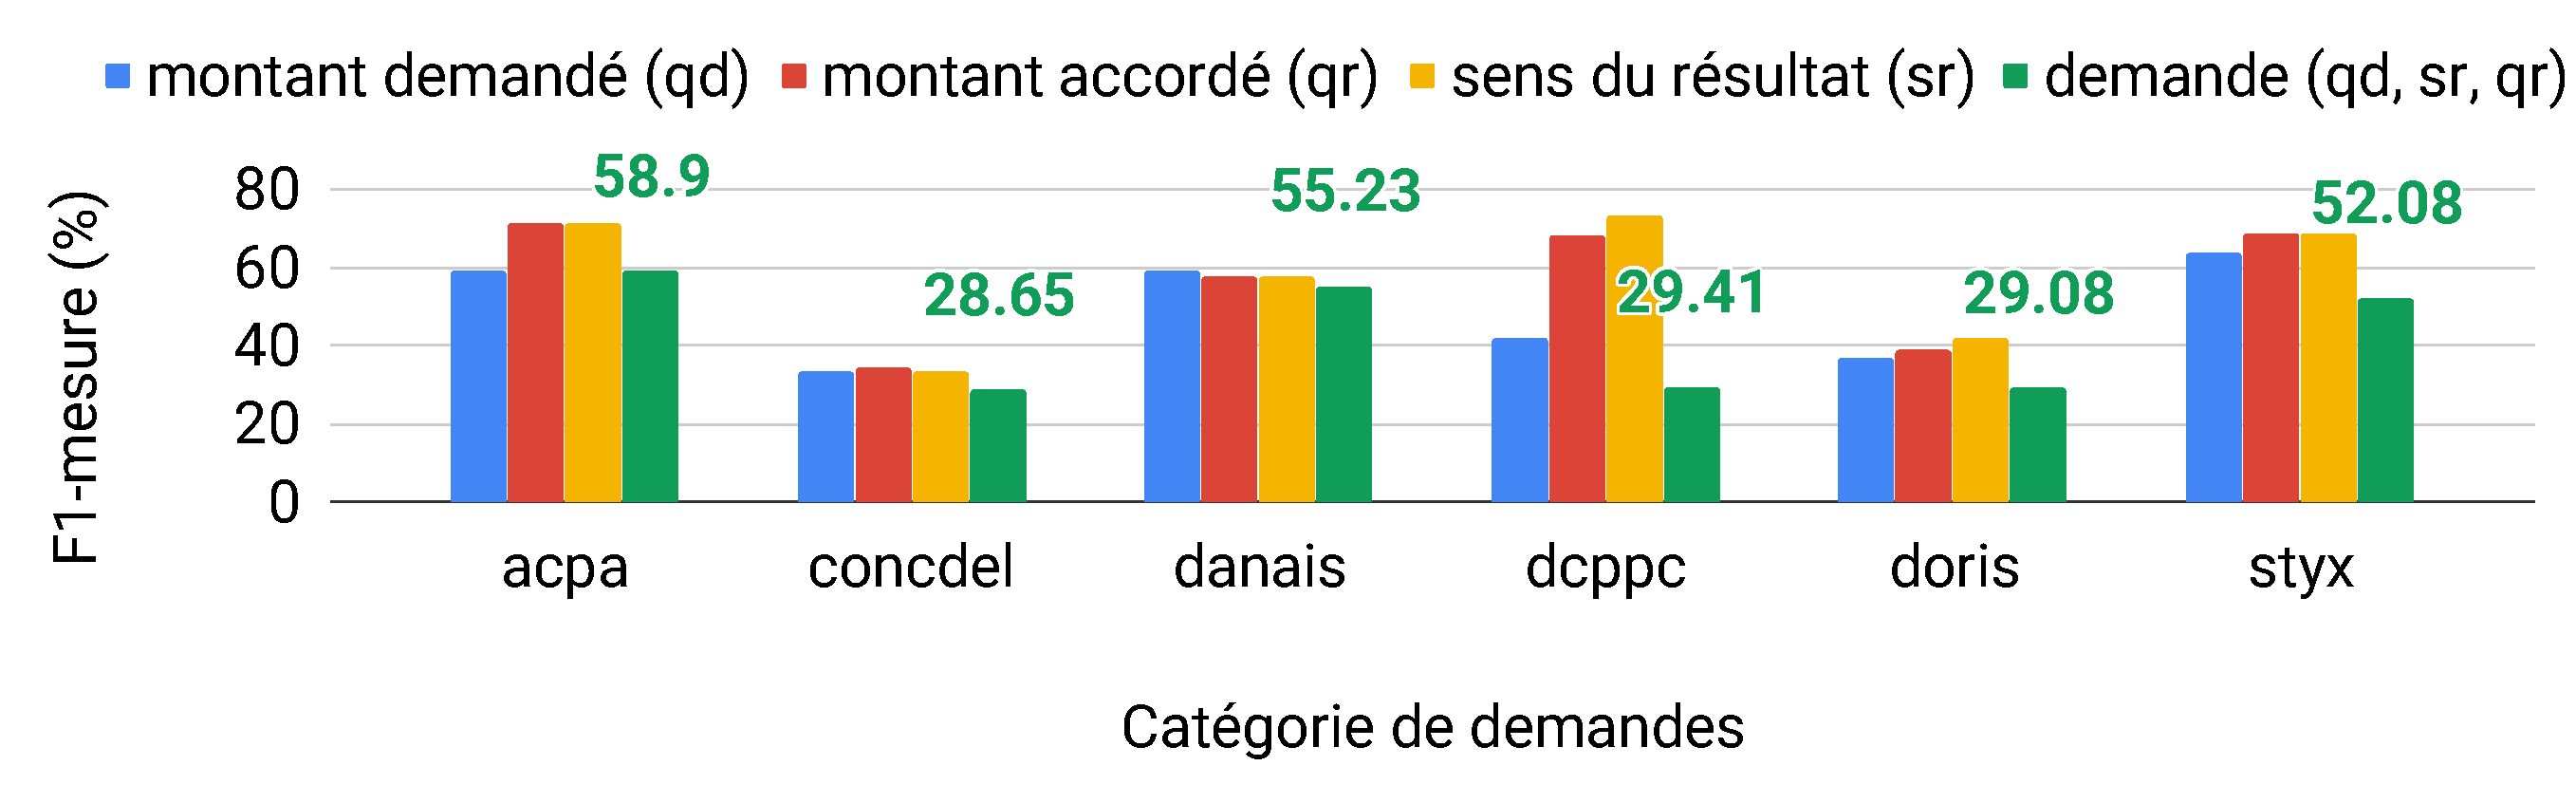
\includegraphics[width=0.9\textwidth]{f1-quanta-et-sens.pdf}}}
		\begin{itemize} \scriptsize
			\item Le résultat est plus accessible 
			\item Certaines catégories (\textit{acpa, danais, styx}) sont plus accessibles que d'autres (\textit{concdel, dcppc, doris})
		\end{itemize}				
		\item Sources d'erreurs:
		\begin{itemize} \scriptsize
			\item Difficulté à identifier les termes-clés rares
			\item Absence de certains quanta dans les énoncés de demandes et résultats
			\item Erreur de mise en correspondance des données extraites
		\end{itemize}
	\end{itemize}
\end{frame}
